\uuid{G4xy}
\exo7id{7102}
\titre{exo7 7102}
\auteur{megy}
\organisation{exo7}
\datecreate{2017-01-21}
\isIndication{true}
\isCorrection{true}
\chapitre{Géométrie affine euclidienne}
\sousChapitre{Géométrie affine euclidienne du plan}
\module{Géométrie}
\niveau{L2}
\difficulte{}

\contenu{
\texte{
% Tags :  carré, rotation
On se donne un carré, et on cherche à construire un carré de même centre, aux côtés parallèles, et d'aire deux fois plus petite, comme ci-dessous:

\begin{center}
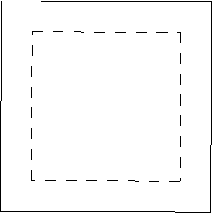
\includegraphics{../images/pdf/G4xy-1.pdf}
\end{center}
}
\begin{enumerate}
    \item \question{(Question préliminaire) Soit $\mathcal C$ un cercle. Montrer qu'un carré circonscrit au cercle a une aire deux fois plus grande qu'un carré inscrit dans le cercle.}
    \item \question{En déduire une solution au problème initial.}
\reponse{
En suivant l'indication on comprend qu'un carré inscrit dans un cercle inscrit au carré initial $ABCD$ a une aire deux fois plus petite que $ABCD$.

\begin{center}
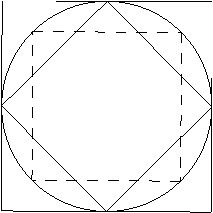
\includegraphics{../images/pdf/G4xy-2.pdf}
\end{center}


On en déduit une construction du petit carré : ses sommets sont les points d'intersection des diagonales avec le cercle inscrit.
}
\indication{Faire tourner le carré circonscrit par rapport au carré inscrit.}
\end{enumerate}
}
